%==================================================================
% BAB 4 HASIL DAN PEMBAHASAN
% Berisi contoh penyajian tabel, gambar, grafik, dan kode program.
%==================================================================
\chapter{HASIL DAN PEMBAHASAN}
\label{chap:hasil}

%------------------------------------------------------------------
\section{Hasil Akuisisi Data}
%------------------------------------------------------------------

Pengambilan data menghasilkan 300 citra ikan bandeng yang terbagi ke
dalam tiga kelas kesegaran. Sebaran jumlah citra setiap kelas
disajikan pada \cref{tab:sebarandata}.

\begin{table}[H]
\caption{Sebaran Jumlah Citra Setiap Kelas Kesegaran}
\label{tab:sebarandata}
\begin{spacing}{1}
\centering
\begin{tabular}{|>{\centering\arraybackslash}p{0.8cm}|>{\raggedright\arraybackslash}p{4.6cm}|>{\centering\arraybackslash}p{2.4cm}|>{\centering\arraybackslash}p{2.8cm}|}
\hline
\rowcolor{blue!12}
\textbf{No} & \textbf{Kelas Kesegaran} & \textbf{Jumlah Citra} & \textbf{Proporsi} \\
\hline
1 & Segar         & 100 & 33,33\% \\
\hline
2 & Cukup segar   & 100 & 33,33\% \\
\hline
3 & Tidak segar   & 100 & 33,33\% \\
\hline
\multicolumn{2}{|c|}{\textbf{Jumlah}} & \textbf{300} & \textbf{100\%} \\
\hline
\end{tabular}
\par\vspace{2pt}
\raggedright\noindent Sumber: hasil pengambilan data (2024)
\end{spacing}
\end{table}

%------------------------------------------------------------------
\section{Hasil Ekstraksi Ciri Warna}
%------------------------------------------------------------------

Nilai rata-rata komponen \textit{hue} pada setiap kelas menunjukkan pola
yang berbeda. Kelas segar memiliki nilai $H$ tertinggi karena warna
insang masih merah cerah, sedangkan kelas tidak segar memiliki nilai
$H$ terendah akibat perubahan warna menuju kecoklatan. Perbandingan
nilai tersebut disajikan pada \cref{fig:ratahue}.

\begin{figure}[H]
\centering
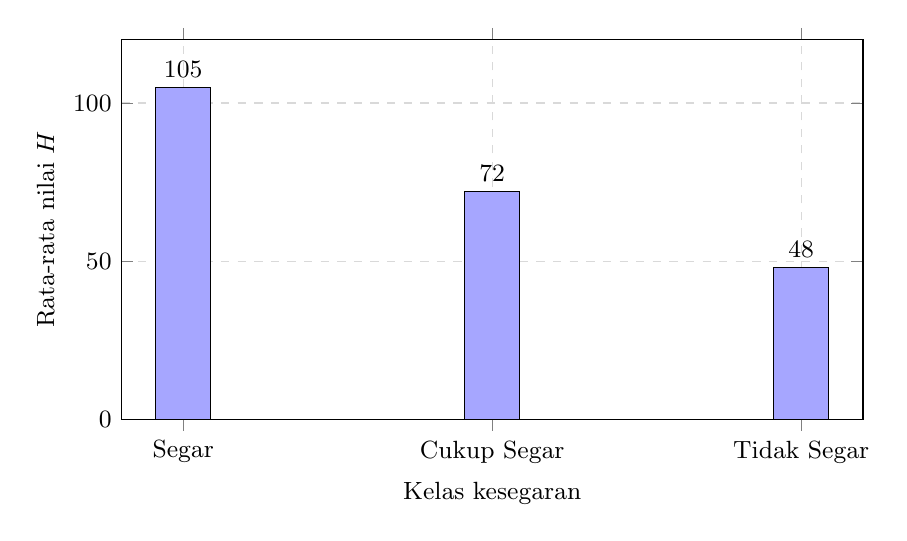
\begin{tikzpicture}
\begin{axis}[
    width=11cm, height=6.4cm,
    ybar, bar width=20pt,
    ymin=0, ymax=120,
    ylabel={Rata-rata nilai $H$},
    xlabel={Kelas kesegaran},
    symbolic x coords={Segar, Cukup Segar, Tidak Segar},
    xtick=data,
    nodes near coords,
    every node near coord/.append style={font=\small},
    grid=major,
    grid style={dashed, gray!30},
    tick label style={font=\small},
    label style={font=\small},
    axis line style={black}
]
\addplot[fill=blue!35, draw=black] coordinates {
    (Segar,105) (Cukup Segar,72) (Tidak Segar,48)
};
\end{axis}
\end{tikzpicture}
\caption{Rata-Rata Nilai \textit{Hue} pada Setiap Kelas Kesegaran Ikan (Hasil Penelitian, 2024)}
\label{fig:ratahue}
\end{figure}

Proses ekstraksi ciri dilakukan menggunakan fungsi bawaan pustaka
OpenCV seperti ditunjukkan pada \cref{lst:ekstraksi}.

\begin{lstlisting}[language=Python, caption={Fungsi Ekstraksi Ciri Warna pada Ruang HSV}, label={lst:ekstraksi}]
def ekstraksi_ciri(path_citra):
    citra = cv2.imread(path_citra)
    citra = cv2.resize(citra, (256, 256))
    hsv = cv2.cvtColor(citra, cv2.COLOR_BGR2HSV)

    ciri = []
    for kanal in cv2.split(hsv):
        ciri.append(float(np.mean(kanal)) / 255.0)
        ciri.append(float(np.std(kanal)) / 255.0)
    return np.array(ciri, dtype=np.float32)
\end{lstlisting}

%------------------------------------------------------------------
\section{Hasil Pelatihan Model}
%------------------------------------------------------------------

Pelatihan dilakukan sebanyak 200 epoch dengan laju pembelajaran 0,01
dan laju penurunan galat yang dinyatakan pada \cref{eq:galat}. Grafik
penurunan galat selama pelatihan disajikan pada \cref{fig:galat}.

\begin{figure}[H]
\centering
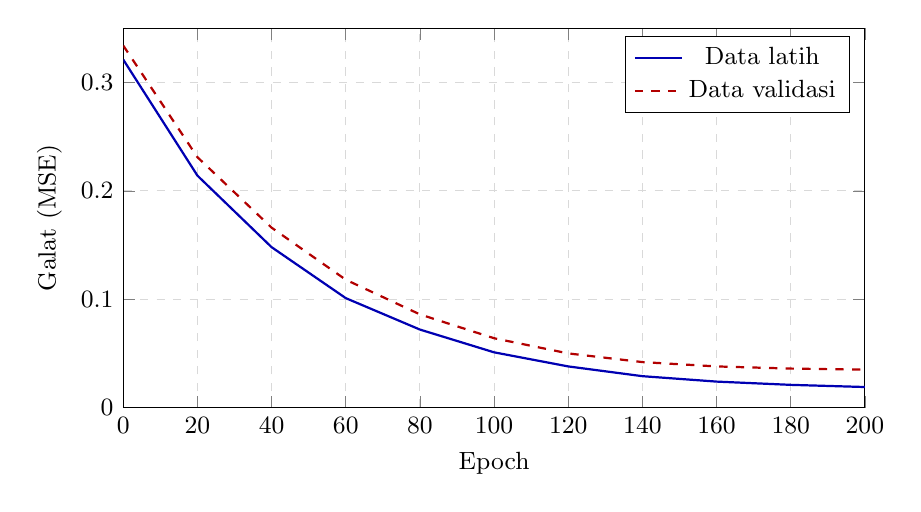
\begin{tikzpicture}
\begin{axis}[
    width=11cm, height=6.4cm,
    xlabel={Epoch},
    ylabel={Galat (MSE)},
    xmin=0, xmax=200,
    ymin=0, ymax=0.35,
    grid=major,
    grid style={dashed, gray!30},
    tick label style={font=\small},
    label style={font=\small},
    legend style={font=\small, at={(0.98,0.98)}, anchor=north east},
    axis line style={black}
]
\addplot[thick, blue!70!black, mark=none] coordinates {
    (0,0.321) (20,0.214) (40,0.148) (60,0.101) (80,0.072)
    (100,0.051) (120,0.038) (140,0.029) (160,0.024) (180,0.021) (200,0.019)
};
\addlegendentry{Data latih}
\addplot[thick, red!70!black, mark=none, dashed] coordinates {
    (0,0.334) (20,0.231) (40,0.166) (60,0.118) (80,0.086)
    (100,0.064) (120,0.050) (140,0.042) (160,0.038) (180,0.036) (200,0.035)
};
\addlegendentry{Data validasi}
\end{axis}
\end{tikzpicture}
\caption{Penurunan Galat Selama Proses Pelatihan (Hasil Penelitian, 2024)}
\label{fig:galat}
\end{figure}

Galat data latih dan data validasi menurun secara konsisten hingga
epoch ke-200. Selisih galat akhir antara keduanya sebesar 0,016
menunjukkan bahwa model tidak mengalami \textit{overfitting} yang
berarti.

%------------------------------------------------------------------
\section{Hasil Pengujian Sistem}
%------------------------------------------------------------------

Pengujian menggunakan \textit{5-fold cross validation} menghasilkan
matriks konfusi seperti pada \cref{tab:konfusi}. Nilai pada diagonal
utama menunjukkan jumlah data yang berhasil diklasifikasikan dengan
benar.

\begin{table}[H]
\caption{Matriks Konfusi Hasil Pengujian Sistem}
\label{tab:konfusi}
\begin{spacing}{1}
\centering
\begin{tabular}{|>{\raggedright\arraybackslash}p{3.4cm}|>{\centering\arraybackslash}p{2.4cm}|>{\centering\arraybackslash}p{2.4cm}|>{\centering\arraybackslash}p{2.4cm}|}
\hline
\rowcolor{blue!12}
\multirow{2}{*}{\textbf{Kelas Aktual}} & \multicolumn{3}{c|}{\textbf{Kelas Prediksi}} \\
\cline{2-4}
 & \textbf{Segar} & \textbf{Cukup Segar} & \textbf{Tidak Segar} \\
\hline
Segar          & \textbf{95} & 5  & 0  \\
\hline
Cukup segar    & 3  & \textbf{89} & 8  \\
\hline
Tidak segar    & 0  & 7  & \textbf{93} \\
\hline
\end{tabular}
\par\vspace{2pt}
\raggedright\noindent Sumber: hasil pengujian (2024)
\end{spacing}
\end{table}

Berdasarkan \cref{tab:konfusi}, akurasi keseluruhan sistem dihitung
menggunakan \cref{eq:akurasi} dan diperoleh nilai 92,33\%. Nilai
presisi dan perolehan setiap kelas disajikan pada \cref{tab:presisi}.

\begin{table}[H]
\caption{Nilai Presisi dan Perolehan Setiap Kelas}
\label{tab:presisi}
\begin{spacing}{1}
\centering
\begin{tabular}{|>{\raggedright\arraybackslash}p{3.6cm}|>{\centering\arraybackslash}p{2.8cm}|>{\centering\arraybackslash}p{2.8cm}|>{\centering\arraybackslash}p{2.8cm}|}
\hline
\rowcolor{blue!12}
\textbf{Kelas} & \textbf{Presisi} & \textbf{Perolehan} & \textbf{F1-Score} \\
\hline
Segar         & 96,94\% & 95,00\% & 95,96\% \\
\hline
Cukup segar   & 88,12\% & 89,00\% & 88,56\% \\
\hline
Tidak segar   & 92,08\% & 93,00\% & 92,54\% \\
\hline
\textbf{Rata-rata} & \textbf{92,38\%} & \textbf{92,33\%} & \textbf{92,35\%} \\
\hline
\end{tabular}
\par\vspace{2pt}
\raggedright\noindent Sumber: hasil pengujian (2024)
\end{spacing}
\end{table}

%------------------------------------------------------------------
\section{Pembahasan}
%------------------------------------------------------------------

Hasil pengujian menunjukkan bahwa sistem yang dirancang mampu
mengklasifikasikan kesegaran ikan dengan akurasi 92,33\%. Nilai tersebut
lebih tinggi dibandingkan penelitian \citet{prasetyo2021} yang
memperoleh akurasi 88,00\% menggunakan ciri warna RGB. Peningkatan ini
terjadi karena ruang warna HSV memisahkan informasi warna dari
kecerahan, sehingga ciri yang dihasilkan lebih tahan terhadap perubahan
intensitas cahaya \citep{gonzalez2018}.

Kesalahan klasifikasi terbanyak terjadi antara kelas cukup segar dan
tidak segar, yaitu sebanyak 15 citra. Hal ini sejalan dengan temuan
\citet{prasetyo2021} bahwa perbedaan warna insang pada kedua kelas
tersebut relatif kecil dan dipengaruhi oleh lama penyimpanan yang tidak
seragam. Kekeliruan juga dipengaruhi oleh adanya pantulan cahaya pada
permukaan mata ikan yang masih lembap.

Kelas segar memiliki presisi tertinggi karena ciri warna pada kelas
tersebut paling berbeda dibandingkan dua kelas lainnya. Dengan demikian,
sistem ini lebih andal digunakan untuk memisahkan ikan segar dari ikan
yang sudah mengalami penurunan mutu, sedangkan pemisahan antara cukup
segar dan tidak segar masih memerlukan ciri tambahan seperti tekstur
insang.
